%
% teil1.tex -- Mellin-Darstellung
%
% (c) 2026 Jannis Gull, OST Ostschweizer Fachhochschule
%
% !TEX root = ../../buch.tex
% !TEX encoding = UTF-8
%

\section{Von der Dirichlet-Reihe zur Mellin-Darstellung
\label{hankel:section:mellin}}
\kopfrechts{Die Mellin-Darstellung}

Die Dirichlet-Reihe enthält den Faktor $n^{-s}$. 
Für die analytische Fortsetzung ist es günstig, diesen Faktor nicht als Potenz, sondern als Integral zu schreiben. 
Genau diese Verbindung liefert die Gamma-Funktion.

\subsection{Die Gamma-Funktion als Bindeglied}

Für $\operatorname{Re}(s)>0$ ist die Gamma-Funktion, dargestellt in~\refeq{hankel:fig:gamma-reell}, durch
\index{Gamma-Funktion}%
\begin{equation}
\Gamma(s)
=
\int_0^\infty
x^{s-1}e^{-x}
\,dx
\label{hankel:eq:gamma-definition}
\end{equation}
definiert~\cite{hankel:dlmf}. 
Die Integralform der Gamma-Funktion wird in Kapitel~\ref{chapter:gamma} ausführlich beschrieben.
\index{Gamma-Funktion!Integralform}
Am Ursprung verhält sich der Betrag des Integranden wie
$x^{\operatorname{Re}(s)-1}$ und ist deshalb genau für
$\operatorname{Re}(s)>0$ integrierbar. 
Für $x\to\infty$ dominiert der exponentielle Faktor $e^{-x}$ jede feste Potenz von $x$.
Die Konvergenz stellt dort kein Problem dar.

Um den Summanden $n^{-s}$ zu erzeugen, wird nicht direkt
\eqref{hankel:eq:gamma-definition}, sondern das skalierte Integral
\begin{equation}
\int_0^\infty x^{s-1}e^{-nx}\,dx
\label{hankel:eq:skaliertes-gamma-integral}
\end{equation}
betrachtet. 
Mit der Substitution
\begin{equation}
u=nx,
\qquad
x=\frac{u}{n},
\qquad
dx=\frac{du}{n}
\label{hankel:eq:substitution-mellin}
\end{equation}
folgt Schritt für Schritt
\begin{equation}
\begin{aligned}
\int_0^\infty x^{s-1}e^{-nx}\,dx
&=
\int_0^\infty
\biggl(\frac{u}{n}\biggr)^{s-1}
e^{-u}\frac{du}{n}
\\
&=
\frac{1}{n^{s-1}}\frac{1}{n}
\int_0^\infty u^{s-1}e^{-u}\,du
\\
&=
\frac{\Gamma(s)}{n^s}.
\end{aligned}
\label{hankel:eq:gamma-skaliert}
\end{equation}
Der Faktor $n^{-s}$ entsteht also aus der Skalierung der
Integrationsvariablen. 
Da die Gamma-Funktion keine Nullstellen besitzt, kann nach $n^{-s}$ aufgelöst werden:
\begin{equation}
\frac{1}{n^s}
=
\frac{1}{\Gamma(s)}
\int_0^\infty
x^{s-1}e^{-nx}
\,dx.
\label{hankel:eq:n-minus-s-integral}
\end{equation}
Diese Formel ist der entscheidende Übergang von der diskreten Summe zu einer Integraldarstellung.

\subsection{Einsetzen und Vertauschen von Summe und Integral}

Das Einsetzen von \eqref{hankel:eq:n-minus-s-integral} in die Dirichlet-Reihe ergibt zunächst
\begin{equation}
\zeta(s)
=
\frac{1}{\Gamma(s)}
\sum_{n=1}^{\infty}
\int_0^\infty
x^{s-1}e^{-nx}
\,dx.
\label{hankel:eq:summe-von-integralen}
\end{equation}
Der nächste Schritt besteht darin, Summe und Integral zu vertauschen. 
Diese Vertauschung ist nicht rein formal, sondern muss durch absolute Integrierbarkeit gerechtfertigt werden. 
Für $s=\sigma+it$ und $x>0$ gilt
\begin{equation}
|x^{s-1}e^{-nx}|
=
x^{\sigma-1}e^{-nx},
\label{hankel:eq:betrag-integrand}
\end{equation}
weil $|x^{it}|=1$. 
Mit derselben Skalierung wie zuvor erhält man
\begin{equation}
\int_0^\infty x^{\sigma-1}e^{-nx}\,dx
=
\frac{\Gamma(\sigma)}{n^\sigma}.
\label{hankel:eq:betrag-skaliert}
\end{equation}
Somit ist für $\sigma>1$
\begin{equation}
\begin{aligned}
\sum_{n=1}^{\infty}
\int_0^\infty
|x^{s-1}e^{-nx}|\,dx
&=
\sum_{n=1}^{\infty}
\frac{\Gamma(\sigma)}{n^\sigma}
&=
\Gamma(\sigma)\zeta(\sigma)
<\infty.
\end{aligned}
\label{hankel:eq:fubini-majorante}
\end{equation}
Damit sind die Voraussetzungen für den Satz von Fubini erfüllt. 
\index{Satz!von Fubini}%
Summe und Integral dürfen also vertauscht werden:
\begin{equation}
\zeta(s)
=
\frac{1}{\Gamma(s)}
\int_0^\infty
x^{s-1}
\sum_{n=1}^{\infty}e^{-nx}
\,dx.
\label{hankel:eq:integral-der-summe}
\end{equation}
Für jedes $x>0$ ist $0<e^{-x}<1$. 
Die innere Reihe ist daher eine geometrische Reihe mit Quotient $e^{-x}$:
\begin{equation}
\begin{aligned}
\sum_{n=1}^{\infty}e^{-nx}
&=
e^{-x}\sum_{k=0}^{\infty}e^{-kx}
&=
\frac{e^{-x}}{1-e^{-x}}
=
\frac{1}{e^x-1}.
\end{aligned}
\label{hankel:eq:geometrische-reihe}
\end{equation}
Damit folgt für $\operatorname{Re}(s)>1$ die Mellin-Darstellung
\begin{equation}
\boxed{
\Gamma(s)\zeta(s)
=
\int_0^\infty
\frac{x^{s-1}}{e^x-1}
\,dx.
}
\label{hankel:eq:mellin-darstellung}
\end{equation}
Der ursprüngliche Summationsindex $n$ ist vollständig verschwunden. 
Statt einer unendlichen Reihe liegt nun ein einzelnes Integral vor, dessen Singularitäten mit Methoden der Analysis untersucht werden können.

\subsection{Wo die Mellin-Darstellung konvergiert}

Die neue Formel ist noch keine analytische Fortsetzung. 
Um dies zu sehen, werden die beiden Enden des Integrationsintervalls getrennt betrachtet. 
Für $x\to\infty$ gilt
\begin{equation}
\frac{1}{e^x-1}
=
\frac{e^{-x}}{1-e^{-x}}
=
O(e^{-x}),
\label{hankel:eq:unendlich-mellin}
\end{equation}
sodass der Integrand dort für jedes feste $s$ wie in Abbildung~\ref*{hankel:fig:mellin-integrand} ersichtlich exponentiell abfällt. 
Die Einschränkung des Konvergenzgebietes kommt ausschliesslich vom Ursprung.
Dort liefert die Taylor-Entwicklung der Exponentialfunktion

\begin{equation}
e^x-1
=
x+\frac{x^2}{2}+O(x^3),
\qquad x\to0,
\label{hankel:eq:exp-taylor-null}
\end{equation}
und damit
\begin{equation}
\frac{1}{e^x-1}
=
\frac{1}{x}
-
\frac{1}{2}
+
O(x).
\label{hankel:eq:bernoulli-anfang}
\end{equation}
Der essentielle Term des Mellin-Integranden ist daher
\begin{equation}
\frac{x^{s-1}}{e^x-1}
\sim
x^{s-2},
\qquad x\to0.
\label{hankel:eq:mellin-asymptotik-null}
\end{equation}
Das Integral $\int_0^1x^{s-2}\,dx$ konvergiert genau für
$\operatorname{Re}(s)>1$. 
Die Mellin-Darstellung besitzt damit zunächst das gleiche Konvergenzgebiet wie die Dirichlet-Reihe. 
Ihr Vorteil liegt an einer anderen Stelle: Das gesamte Problem ist jetzt in der einzigen Singularität
bei $x=0$ konzentriert.

%
% fig-mellin-integrand.tex
%
% (c) 2026 Prof Dr Andreas Müller
%
\begin{figure}
	\centering
	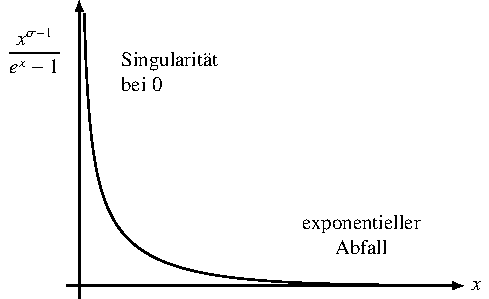
\includegraphics{papers/hankel/images/mellin-integrand.pdf}
%	\begin{tikzpicture}[scale=1.05,>=latex]
%		
%		% Achsen
%		\draw[->] (-0.2,0) -- (6.2,0)
%		node[right] {$x$};
%		
%		\draw[->] (0,-0.2) -- (0,4.6);
%		
%		% Beschriftung der y-Achse bewusst links
%		\node[anchor=east] at (-0.15,3.8)
%		{$\displaystyle\frac{x^{\sigma-1}}{e^x-1}$};
%		
%		% Kurve: nahe genug an x=0 beginnen,
%		% damit der singuläre Anstieg sichtbar wird
%		\begin{scope}
%			\clip (-0.2,-0.2) rectangle (6.2,4.6);
%			\draw[thick,domain=0.08:6,samples=200]
%			plot (\x,{(\x^0.4)/(exp(\x)-1)});
%		\end{scope}
%		
%		% Hinweise
%		\node[align=left,anchor=west] at (0.55,3.45)
%		{Singularität\\bei $0$};
%		
%		\node[align=center] at (4.55,0.82)
%		{exponentieller\\Abfall};
%		
%	\end{tikzpicture}
	\caption{Schematisches Verhalten des Mellin-Integranden für einen festen
		Realteil $1<\sigma<2$. Nur der Ursprung begrenzt das Konvergenzgebiet.}
	\label{hankel:fig:mellin-integrand}
\end{figure}

%\begin{figure}
%	\centering
%	\begin{tikzpicture}[scale=1.05,>=latex]
%		
%		% Achsen
%		\draw[->] (-0.2,0) -- (6.2,0)
%		node[right] {$x$};
%		
%		\draw[->] (0,-0.2) -- (0,4.6);
%		
%		% Beschriftung der y-Achse bewusst links
%		\node[anchor=east] at (-0.15,3.8)
%		{$\displaystyle\frac{x^{\sigma-1}}{e^x-1}$};
%		
%		% Kurve: nahe genug an x=0 beginnen,
%		% damit der singuläre Anstieg sichtbar wird
%		\begin{scope}
%			\clip (-0.2,-0.2) rectangle (6.2,4.6);
%			\draw[thick,domain=0.08:6,samples=200]
%			plot (\x,{(\x^0.4)/(exp(\x)-1)});
%		\end{scope}
%		
%		% Hinweise
%		\node[align=left,anchor=west] at (0.55,3.45)
%		{Singularität\\bei $0$};
%		
%		\node[align=center] at (4.55,0.82)
%		{exponentieller\\Abfall};
%		
%	\end{tikzpicture}
%	\caption{Schematisches Verhalten des Mellin-Integranden für einen festen
%		Realteil $1<\sigma<2$. Nur der Ursprung begrenzt das Konvergenzgebiet.}
%	\label{hankel:fig:mellin-integrand}
%\end{figure}
Genau diese Situation ist die Motivation für den nächsten Schritt. 
Statt den Ursprung auf der reellen Achse zu durchlaufen, wird die Integration in die komplexe Ebene verlegt.
Der singuläre Punkt wird auf einer kleinen Kontur umgangen. 
Dafür muss zuvor geklärt werden, wie die komplexe Potenz $(-z)^{s-1}$ auf beiden Seiten eines Verzweigungsschnittes zu verstehen ist.
